\paragraph{}Esta es la página principal o de inicio de la aplicación web $\mu$Search para el administrador de la misma. A esta página de inicio, el administrador será siempre redirigido cuando pulse en cualquiera de los dos logotipos de la cabecera de la página.

\paragraph{}Se le muestra al administrador un mensaje de bienvenida y una breve descripción las funcionalidades que tiene disponibles como administrador de la aplicación web.

\begin{figure}[h!]
	\centering
	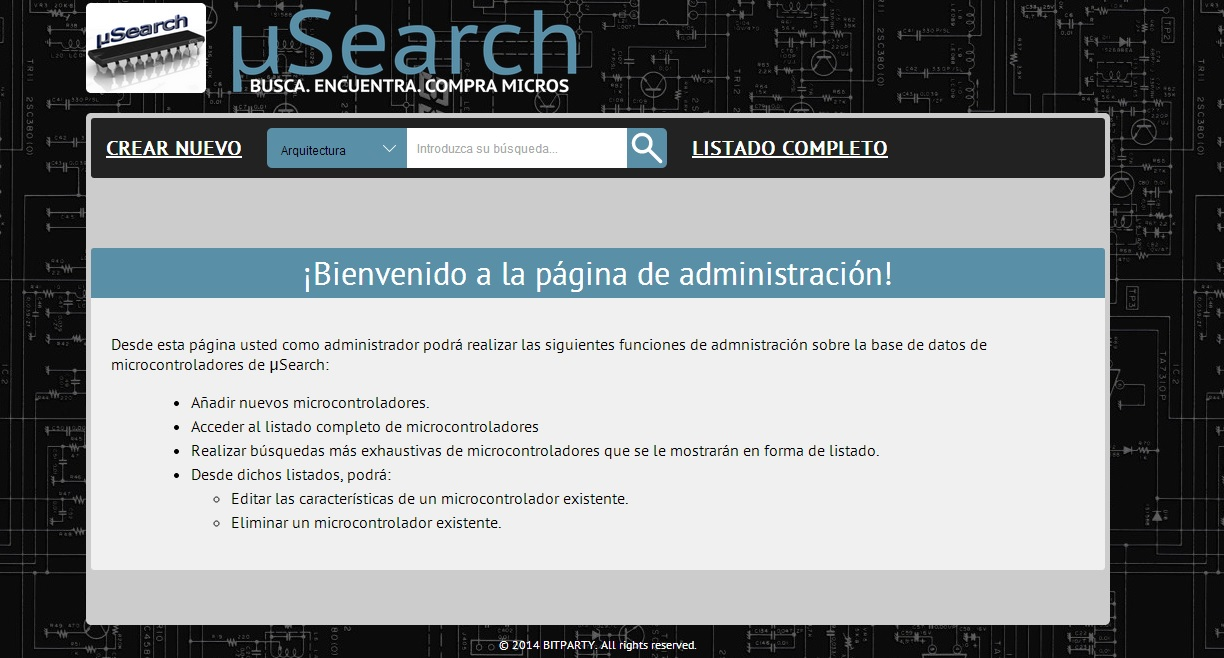
\includegraphics[width=0.85\textwidth]{img/principal_admin}
	\caption{Página principal de administración.}
	\label{fig:principal_admin}
\end{figure}

Desde esta página, a través de los iconos situados en la cabecera debajo de los logotipos de la web, el administrador puede acceder a:
\begin{itemize}
	
	\item \textbf{Crear Nuevo:} Redirige al administrador a la página para añadir un nuevo microcontrolador al catálogo electrónico.
	
	\item \textbf{Búsqueda:} Desde esta sección, el administrador puede realizar búsquedas sobre el catálogo de microcontroladores en base a cualquiera de sus características (Arquitectura, Frecuencia, Flash, RAM). Se debe seleccionar una de las características de la lista despegable, introducir el texto a buscar y pulsar sobre el icono de búsqueda.
	El usuario será redirigido a una página donde se le mostrará el resultado de la búsqueda.
	
	\item \textbf{Listado Completo:} Redirige al administrador a la página en la que se listan todos los microcontroladores disponibles en el catálogo.
	
\end{itemize}